\subsection*{Tæller}
\label{volumenkontrol-simulering-taeller}

Det er tællerens opgave at holde styr på hvad volumenniveauet er. Der tælles op eller ned når der trykkes på én af de to volumenknapper. Hvor hurtigt der skal tælles bestemmes af det AND'ende signal fra VCO'en og XOR-gaten. Tælleren danner også grundlag for hvad der skal stå i displayet.

\subsection*{Display driver}
\label{volumenkontrol-simulering-display_driver}

Display driveren konvertere signalet fra tælleren til et signal der kan vises på de to 7-segment displays. Display driveren er opbygget af digitale gates, for at få flere forskellige slags kredsløb i HiFi-forstærkeren.

\subsection*{Display}
\label{volumenkontrol-simulering-display}

Displayet består af to 7-segment displays, der viser hvor meget signalet er blevet dæmpet, målt i dB.

\subsection*{Dæmper}
\label{volumenkontrol-simulering-daemper}

Dæmperen er en en analog attenuator, der er sammen sat af to sæt modstands attenuatore adskilt af en buffer. Dæmpningen indstilles ved at ændre hvor signalet tages ud af de to modstands attenuatore, dette styres med en analog multiplekser. Den første attenuatorer består af seks modstande hvor der er en dæmpning på 8 dB mellem hver, den anden attenuatorer består af syv modstande hvor der er en dæmpning på 1 dB mellem hver. Det er således muligt at kombinere de to attenuatorer til at dæmpe signalet mellem 0 og 55 dB, med spring af 1 dB. Diagrammet er afbilledet på figur \ref{fig:volumenkontrol_daemper}. Modstandene er beregnet i appendiks C??.

\begin{figure}[h]
\centering
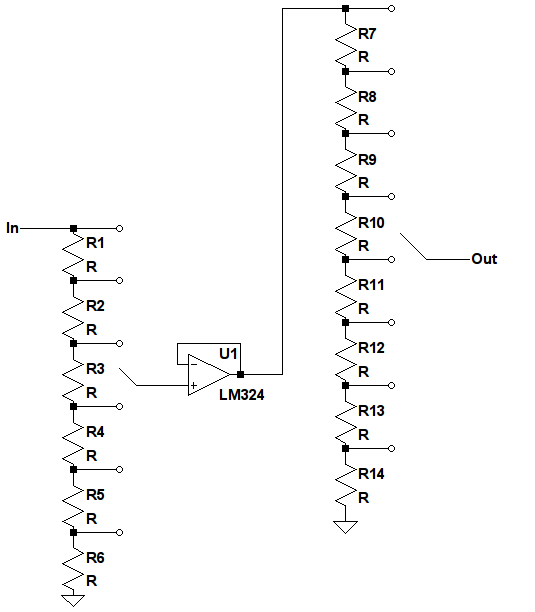
\includegraphics[scale=1]{teknisk/volumenkontrol/daemper.png}
\caption{Diagram over dæmperen}
\label{fig:volumenkontrol_daemper}
\end{figure}

\subsection*{Simulering}
\label{volumenkontrol-simulering}

\section{Accepttest}
\label{volumenkontrol-accepttest}

